% (The MIT License)
%
% Copyright (c) 2023-2024 Yegor Bugayenko
%
% Permission is hereby granted, free of charge, to any person obtaining a copy
% of this software and associated documentation files (the 'Software'), to deal
% in the Software without restriction, including without limitation the rights
% to use, copy, modify, merge, publish, distribute, sublicense, and/or sell
% copies of the Software, and to permit persons to whom the Software is
% furnished to do so, subject to the following conditions:
%
% The above copyright notice and this permission notice shall be included in all
% copies or substantial portions of the Software.
%
% THE SOFTWARE IS PROVIDED 'AS IS', WITHOUT WARRANTY OF ANY KIND, EXPRESS OR
% IMPLIED, INCLUDING BUT NOT LIMITED TO THE WARRANTIES OF MERCHANTABILITY,
% FITNESS FOR A PARTICULAR PURPOSE AND NONINFRINGEMENT. IN NO EVENT SHALL THE
% AUTHORS OR COPYRIGHT HOLDERS BE LIABLE FOR ANY CLAIM, DAMAGES OR OTHER
% LIABILITY, WHETHER IN AN ACTION OF CONTRACT, TORT OR OTHERWISE, ARISING FROM,
% OUT OF OR IN CONNECTION WITH THE SOFTWARE OR THE USE OR OTHER DEALINGS IN THE
% SOFTWARE.

\documentclass{article}
\usepackage{../lecture-notes/notes}
\usepackage{setspace}
\newcommand*\thetitle{-ER}
\newcommand*\thesubtitle{Alternatives, Clients, MVC}
\begin{document}

\plush{\lnTitlePage{5}{8}{6GMiosTLUTc}}

\pptToc

\lnQuote
  {carlo-pescio}
  {When you need a \ul{manager}, it’s often a sign that the \ul{managed} are just plain old data structures and that the manager is the smart procedure doing the real work.}
  {pescio2011your}

\plush{\pptChapter[Alternatives]{Examples and Alternatives}}

\pptSection{Parser}
\begin{pptWide}{2}
{\small\begin{ffcode}
class Parser {
  static int parseInt(String t) {
    // Parse String into Integer
  }
  static float parseFloat(String t) {
    // Parse String into Float
  }
  // And many more methods...
}

int x = Parser.parseInt("42");
\end{ffcode}
}
\par\columnbreak\par
{\small\begin{ffcode}
class StringAsInt implements Number {
  private final String txt;
  StringAsInt(String t) { this.txt = t; }
  @Override int intValue() {
    // Parse String into Integer
    // and return the value
  }
}

Number n = new StringAsInt("42");
int x = n.intValue();
\end{ffcode}
}
\end{pptWide}
\plush{}

\pptSection{Reader}
\begin{pptWide}{2}
{\small\begin{ffcode}
class Reader {
  static char readChar(InputStream i) {
    // Read the next char from the
    // stream and return it, or NULL
    // if the stream is at the EOF
  }
}

InputStream i = new FileInputStream(..);
char c = Reader.readChar(i);
\end{ffcode}
}
\par\columnbreak\par
{\small\begin{ffcode}
class Chars
  private final InputStream is;
  Chars(InputStream i)
    this.is = i;
  char next()
    // Read the next char from the
    // stream and throw exception
    // if !exists()
  bool exists()
    // Return TRUE if not EOF
InputStream i = new FileInputStream(..);
Chars chars = new Chars(i);
char c = chars.next();
\end{ffcode}
}
\end{pptWide}
\plush{}

\pptSection{Controller}
\begin{pptWide}{2}
{\small\begin{ffcode}
class SimpleController {
  @GET
  @Path("/index")
  HttpResponse index(HttpRequest e) {
    // Build an index page and return
  }
  @POST
  @Path("/update")
  HttpResponse update(HttpRequest e) {
    // Save new user information
    // and return HTTP 303
  }
}
\end{ffcode}
}
\par\columnbreak\par
{\small\begin{ffcode}
class IndexPage implements HttpPage
  HttpResponse process(HttpRequest e) {
    // Build an index page and return
  }
class UpdatePage implements HttpPage
  HttpResponse process(HttpRequest e) {
    // Save new user information
    // and return HTTP 303
  }
new AllPages(
  new IndexPage(),
  new UpdatePage()
);
\end{ffcode}
}
\end{pptWide}
\plush{}

\pptSection{Validator}
\begin{pptWide}{2}
{\small\begin{ffcode}
class Validator {
  bool isValid(int age) {
    return age >= 18;
  }
}
int a = 23;
Validator v = new Validator();
if (!v.isValid(a)) {
  throw new Exception(
    "Age is not valid"
  );
}
\end{ffcode}
}
\par\columnbreak\par
{\scriptsize\begin{ffcode}
interface Age
  int value();
class DefaultAge implements Age
  private final int a;
  DefaultAge(int a)
    this.a = a;
  @Override int value()
    return this.a;
class ValidAge implements Age {
  private final Age origin;
  ValidAge(Age age)
    this.origin = age;
  @Override int value()
    int v = this.origin.value();
    if (v < 18)
      throw new Exception("Age is not valid");
    return v;
Age a = new ValidAge(new DefaultAge(23));
\end{ffcode}
}
\end{pptWide}
\plush{}

\pptSection{Encoder}
\begin{pptWide}{2}
{\scriptsize\begin{ffcode}
package java.net;

class URLEncoder {
  static String encode(String s, String enc) {
    // Encode the string "s" using
    // the "enc" encoding and return
    // the encoded string
  }
}
String e = URLEncoder.encode("@foo");
e.equals("%40foo");
\end{ffcode}
}
You may want to read more about this in
my blog~\citep{bugayenko2015blog0309,bugayenko2017blog0912}.
\par\columnbreak\par
{\scriptsize\begin{ffcode}
class Encoded implements String {
  private final String origin;
  private final String encoding;
  Encoded(String s, String enc) {
    this.origin = s;
    this.enc = encoding;
  }
  @Override String value() {
    // Encode the string "origin" using
    // the "encoding" and return
    // the encoded string
  }
}
String e = new Encoded("@foo");
e.value().equals("%40foo");
\end{ffcode}
}
\end{pptWide}
\par
The right snippet won't work in Java, since \ff{String} is a final class, not an interface, unfortunately.
\plush{}

\plush{\pptSection[Proof]{Proof: Classes with -ER Suffixes Are More Complex}
  \begin{multicols}{2}
  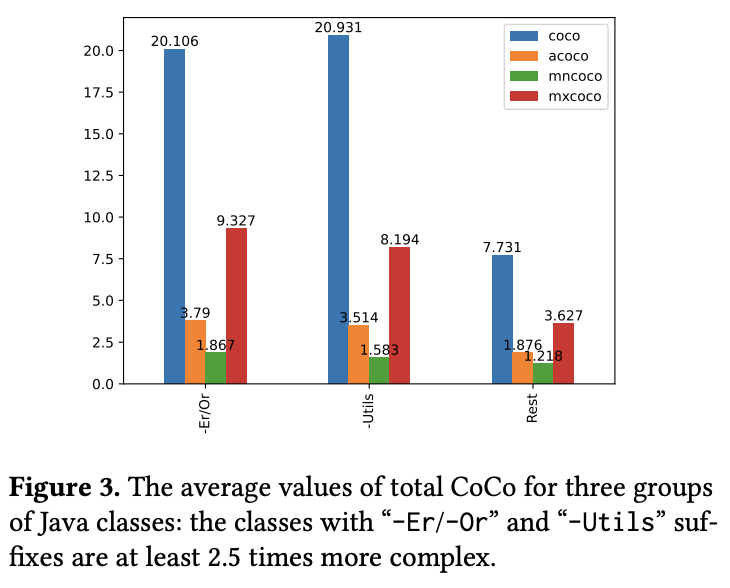
\includegraphics[width=\linewidth]{er.png}
  \par\columnbreak\par
  \begin{spacing}{0.9}
  ``We took 13,861 Java classes from 212 open source repositories, divided them into three groups (`-Er' classes, `-Utils', and others), and evaluated their complexity. Because average CC and CoCO in the first two groups were almost 3x larger than in the third group, we concluded that functor classes may be considered \ul{bad design}.''
  \end{spacing}
  \par
  \lnSource{sukhova2024java}
  \end{multicols}}

\plush{\pptChapter[-Client]{-Client Suffix}}

\pptSection[AWS]{AWS Java Client}
\begin{pptWide}{2}
{\scriptsize\begin{ffcode}
class AmazonS3Client {
  createBucket(String name);
  deleteBucket(String name);
  doesBucketExist(String name);
  getBucketAcl(String name)
  getBucketPolicy(String name);
  listBuckets();
  // 160+ more methods here
}
client = new AmazonS3Client("us-1");
client.createBucket("foo");
client.putObject("foo", "a.txt");
client.writeObject("foo", "a.txt", "data");
\end{ffcode}
}
\par\columnbreak\par
{\scriptsize\begin{ffcode}
region = new S3Region("us-1");
bucket = region.createBucket("foo");
object = bucket.putObject("a.txt");
object.write("data");
\end{ffcode}
}
It's here: \href{https://github.com/jcabi/jcabi-s3}{jcabi/jcabi-s3}.
\end{pptWide}
\par
The left snippet is:
\begin{inparaenum}[1)]
\item procedural,
\item hard to test,
\item resembles a utility class,
and
\item is hard to extend.
\end{inparaenum}
The right one is object-oriented.
\plush{}

\plush{\pptChapter[Performance]{What About Performance?}}

\pptSection[Sticky]{Sticky Parseable Object}
\begin{pptWide}{2}
{\small\begin{ffcode}
class StringAsInt implements Number {
  private final String txt;
  StringAsInt(String t) { this.txt = t; }
  @Override int intValue() {
    // Parse String into Integer
    // and return the value
  }
}

Number n = new StringAsInt("42");
int x = n.intValue();
\end{ffcode}
}
\par\columnbreak\par
{\small\begin{ffcode}
class StickyInt implements Number {
  private final Number origin;
  private int cache = 0;
  private bool cached = false;
  StickyInt(Number n) { origin = n; }
  @Override int intValue() {
    if (!cached) {
      cache = origin.intValue();
      cached = true;
    }
    return cache; } }
\end{ffcode}
}
\end{pptWide}
\par
Is it thread-safe though?
\plush{}

\pptSection[Safe]{Thread-safe Sticky Parseable Object}
\begin{pptWide}{2}
{\small\begin{ffcode}
class StickyInt implements Number {
  private final Number origin;
  private int cache = 0;
  private bool cached = false;
  StickyInt(Number n) { origin = n; }
  @Override int intValue() {
    if (!cached) {
      cache = origin.intValue();
    }
    return cache;
  }
}
\end{ffcode}
}
\par\columnbreak\par
{\scriptsize\begin{ffcode}
class StickyInt implements Number {
  private final Number origin;
  private final AtomicReference<Integer> cache =
    new AtomicReference<Integer>(null);
  StickyInt(Number n) { origin = n; }
  @Override int intValue() {
    return cache.updateAndGet(
      x -> {
        if (x == null) {
          return origin.intValue();
        }
        return x;
      }
    );
  }
}
\end{ffcode}
}
\end{pptWide}
\par
The left snippet is not thread-safety, while the right one is.
\plush{}

\plush{\pptChapter[MVC]{Model-View-Controller (MVC)}}

\pptSection[Controller]{The Controller}
\begin{pptWide}{2}
{\small\begin{ffcode}
class Controller {
  @GET
  @Path("/b{id}")
  String index(int id) {
    Book book = em.findById(id);
    View v = new HtmlView("book.html");
    v.set("title", book.getTitle());
    return v.renderHtml();
  }
}
\end{ffcode}
}
\par\columnbreak\par
\pptPic{0.7}{mvc.png}\par
This is bad OOP~\citep{bugayenko2016blog1213}.
\end{pptWide}
\par
\plush{}

\pptSection[HTML]{Book as HTML}
\begin{pptWide}{2}
{\small\begin{ffcode}
class Controller {
  @GET
  @Path("/b{id}")
  String index(int id) {
    Book book = em.findById(id);
    View v = new HtmlView("book.html");
    v.set("title", book.getTitle());
    return v.renderHtml();
  }
}
\end{ffcode}
}
\par\columnbreak\par
{\scriptsize\begin{ffcode}
interface Book
  String title();
class PgBook implements Book
  String title() // loads from PostgreSQL
interface Page
  String html();
class HtmlBook implements Book, Page
  String html() // renders in HTML
  String title() // returns origin.title()
class PageOnPath implements Page
  private final String path;
  private final Page origin;
  String html() // renders if path matches
\end{ffcode}
}
\end{pptWide}
\par
Check \href{https://github.com/yegor256/jpages}{yegor256/jpages} and \href{https://github.com/yegor256/takes}{yegor256/takes}.
\plush{}

\plush{\begin{pptMiddle}
  \pptChapter[Takes]{Rultor + Takes}
  \par
  \begin{tabular}{lp{2em}l}
    
\includegraphics[height=1.6in]{rultor.png} & & 
\includegraphics[height=1.6in]{takes.png} \\
    \href{https://www.rultor.com}{\texttt{rultor.com}} & & \href{https://www.takes.org}{\texttt{takes.org}} \\
  \end{tabular}
\end{pptMiddle}}

\plush{\begin{multicols}{2}
  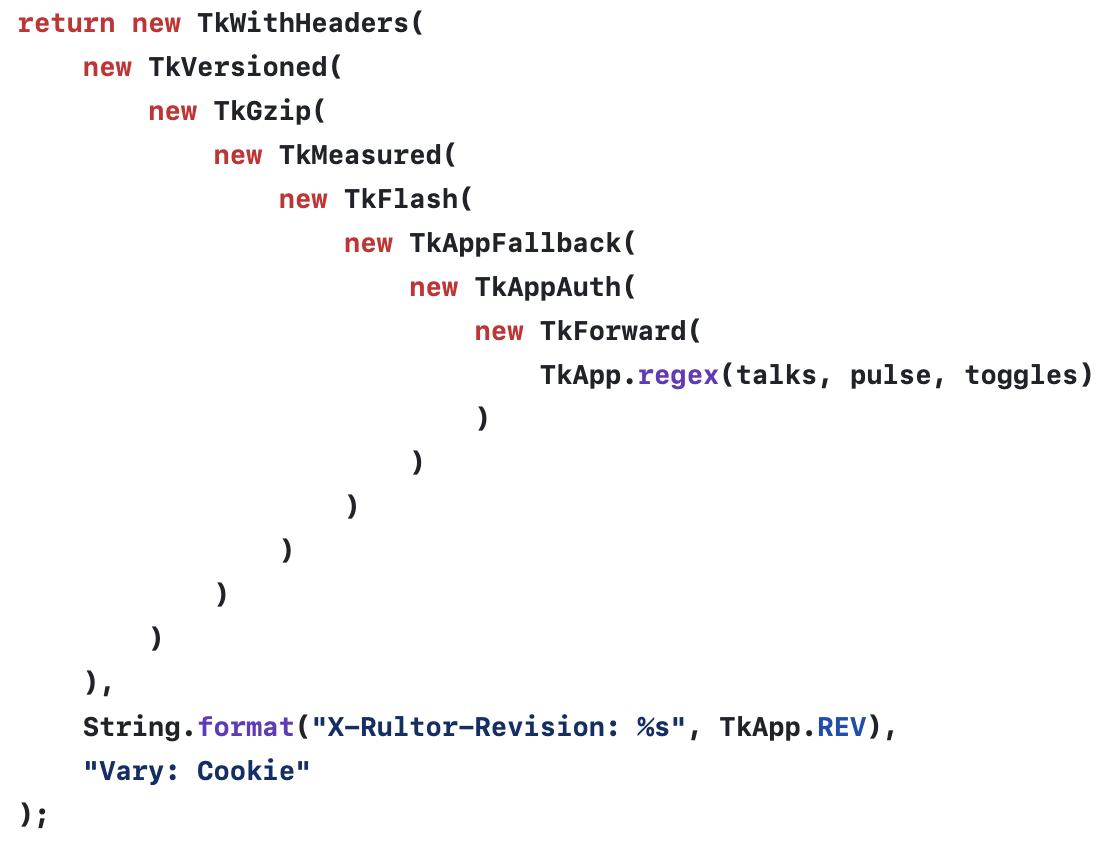
\includegraphics[width=.9\linewidth]{rultor-1.png}
  \par\columnbreak\par
  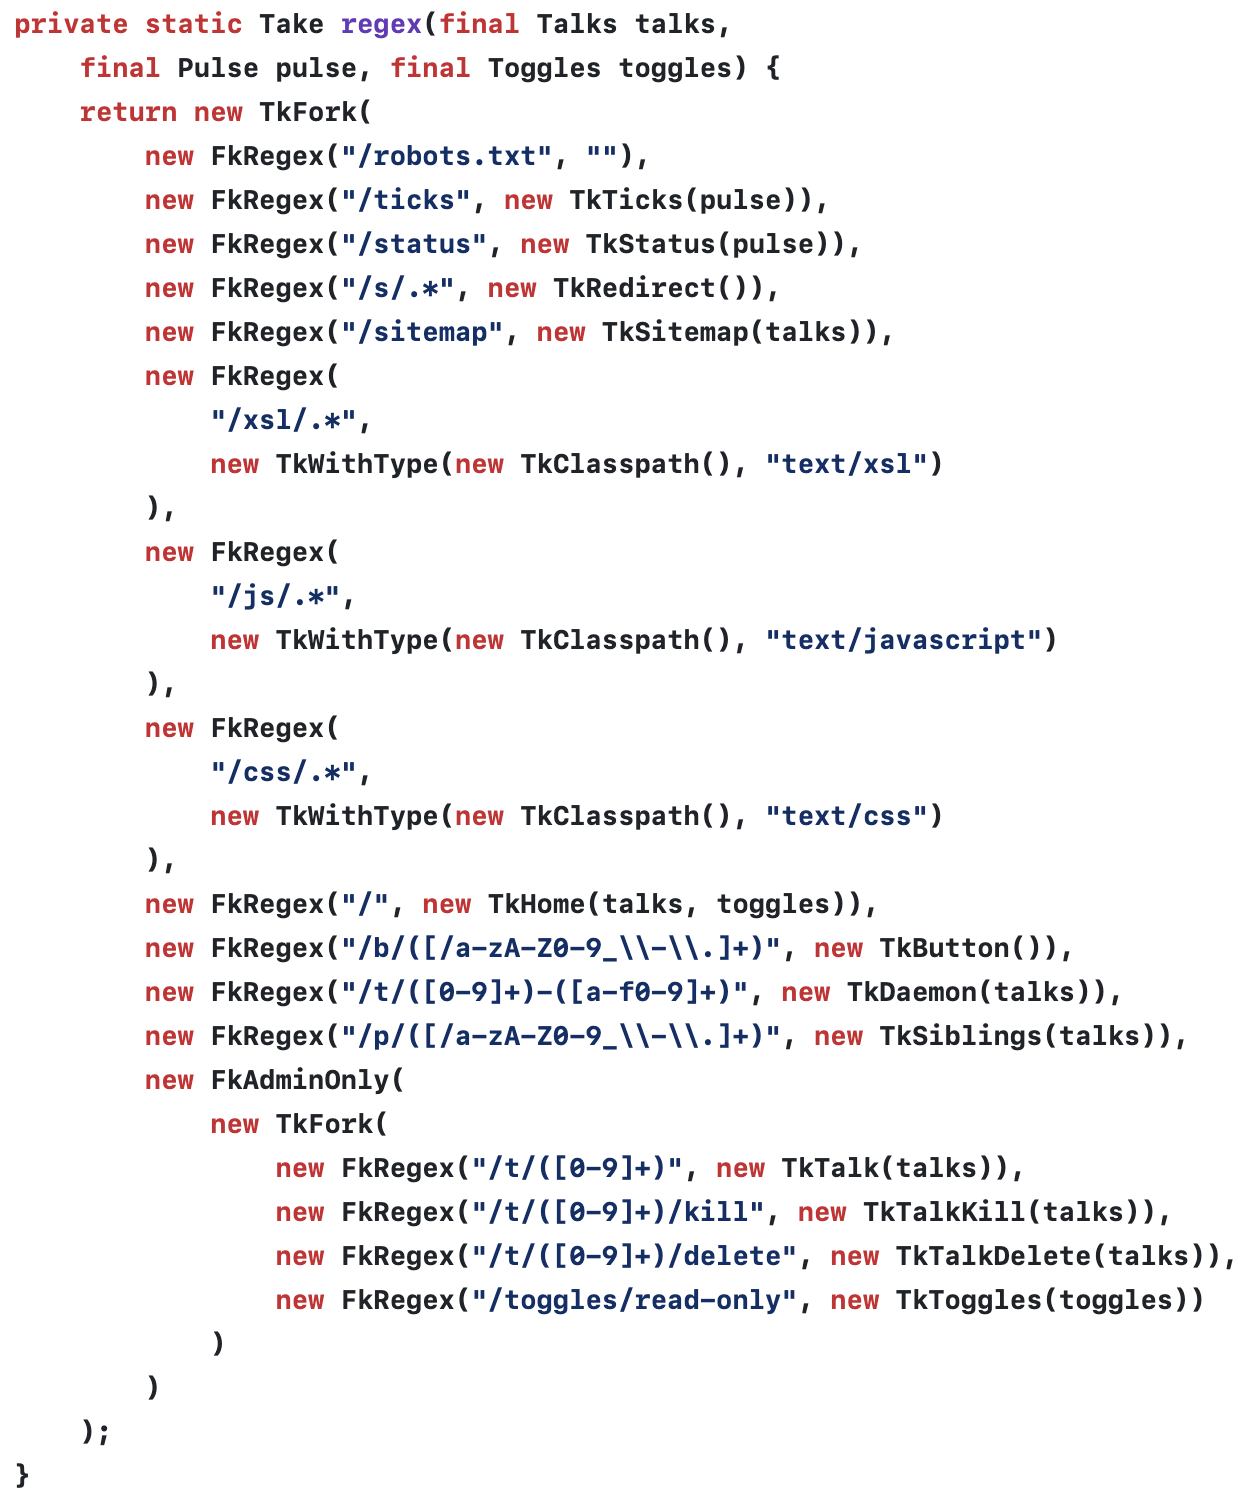
\includegraphics[width=.9\linewidth]{rultor-2.png}
  \end{multicols}\par
  {\tiny \url{https://github.com/yegor256/rultor/blob/master/src/main/java/com/rultor/web/TkApp.java}\par}}

\end{document}
